\documentclass{article} 
\RequirePackage{amssymb} 
\RequirePackage{amsmath}
\usepackage[latin1]{inputenc} 
\usepackage{graphicx}

\title{Esercizio 5 di riepilogo} 
\author{Davide Angelocola} 

\begin{document}
\maketitle

\section{Testo del problema} 
Un'apparecchiatura di et� $j \ge 0$ all'inizio della giornata si guasta
durante la giornata con probabilit� $p_j$ e in tal caso � sostituita
da un'apparecchiatura identica ma nuova, che entra in funzione
all'inizio della giornata successiva. L'apparecchiatura � sostituita anche quando � troppo vecchia e si conviene che questo corrisponda all'et� N (per et� di un'apparecchiatura si intende qui
il numero delle giornate intere in cui l'apparecchiatura ha funzionato). Per $n \ge 0$, si indica con $X_n$ la v.a. che conta l'et�
dell'apparecchiatura funzionante all'inizio della $n$+1-ma giornata.

\begin{itemize} 
 \item i) Scrivi la matrice di transizione della catena di Markov $(X_n)_{n} \ge 0 $ e determina il carattere degli stati.
 \item ii) Se al tempo $n = 0$ l'apparecchiatura � nuova, con che probabilit� � nuova al tempo $n = 2$?
\end{itemize} 

\section{punto i)} 

Se $p_j$ � la probabilit� che al giorno $j$ l'apparacchiatura si rompa, allora $q_j = 1- p_j$ rappresenta la probabilit� di non rottura. Ogni stato rappresenta un giorno passato senza guasti. Ad esempio il giorno 3 rappresenta 3 giorni consecutivi senza guasti. Lo stato $j=0$ invece rappresenta un "guasto", ovvero un guasto e una sostituzione, con 0 giorni di "uptime". L'ultimo stato rappresenta lo stato "troppo vecchio" (et� N).

Proviamo a disegnare il problema con un grafo delle transizioni:

%%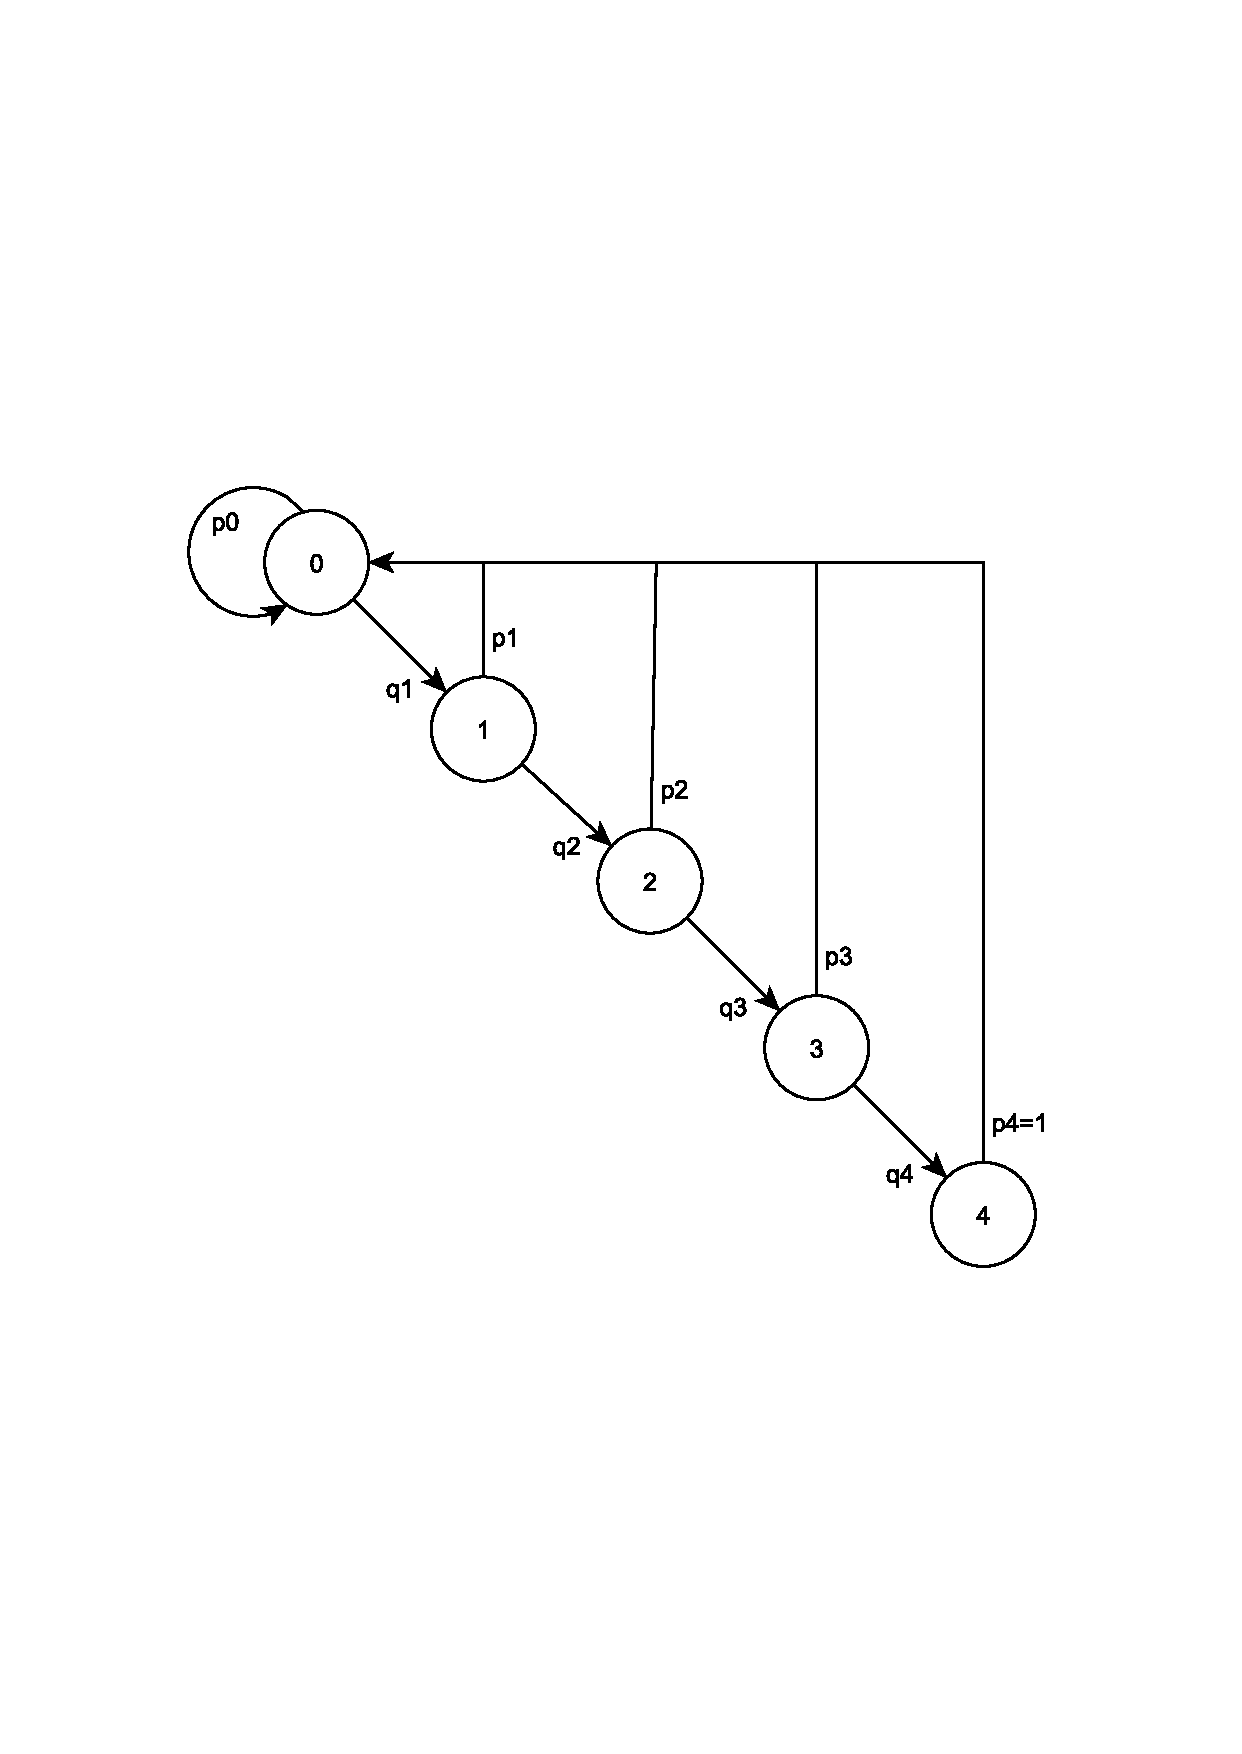
\includegraphics[scale=0.40]{cp_ex5_fig1.pdf} 

Come si evince dal grafo si torna nello stato 0 con probabilit� $p_j$, si va invece "al giorno successivo" con probabilit� $q_j$. Una volta raggiunta l'et� $N$ si obbliga la sostituzione ($p_N = 1$).

Gli stati quindi sono tutti transienti?

\section{punto ii)} 

Intuitivamente guardando il grafo vediamo che sono possibili due percorsi:

\begin{itemize} 
  \item due rotture di seguito, che avvengono con probabilit� $p_0 p_0 = p_0^2$  
  \item un giorno senza guasti, che avviene con probabilit� $q_0$, e un una rottura al secondo giorno, che avviene con probabilit� $p_1$   
\end{itemize}  

al secondo giorno avremo un'apparecchiatura nuova con probabilit�:
$$
p_0^2 + p_1q_0
$$

Avremmo potuto anche usare la matrice di transizione (con N fissato a 4, come nel grafo sopra):

$$
P = \begin{pmatrix} 
p_0 & q_0 & 0   & 0   & 0   \cr 
p_1 & 0   & q_1 & 0   & 0   \cr 
p_2 & 0   & 0   & q_2 & 0   \cr 
p_3 & 0   & 0   & 0   & q_3 \cr 
1   & 0   & 0   & 0   & 0   \cr 
\end{pmatrix} 
$$

in due passi si ottiene:

$$
\pi _2 = 
\begin{pmatrix} 
p_0^2 + p_1 q_0  &  p_0   q_0  &  q_0   q_1  & 0 & 0 \cr 
p_0 p_1 + p_2   q_1  &  p_1   q_0  & 0 &  q1   q_2  & 0 \cr 
p_0 p_2 + p_3   q_2  &  p_2   q_0  & 0 & 0 &  q_2   q3  \cr
p_0 p_3 + q_3  &  p_3   q_0  & 0 & 0 & 0 \cr 
p_0 & q_0 & 0 & 0 & 0 \cr
\end{pmatrix}
$$

La probabilit� cercata � $$P^2_{0 0} = p_0^2 + p_1 q_0$$.

\end{document}
